\begin{center}
\Large \textbf{Problema 4}
\end{center}

Una diagonal en un polígono regular es cualquier segmento de línea que conecta dos vértices no adyacentes del polígono.
En otras palabras, es una línea recta que une dos esquinas del polígono que no están directamente conectadas por un lado.

\begin{figure}[H]
    \centering
    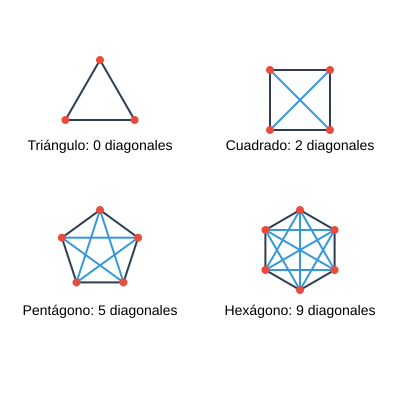
\includegraphics[width=0.5\textwidth]{diagonales.png}
\end{figure}

\underline{¿Cuántas diagonales tiene un polígono regular de $2025$ lados?}

